\begin{dang}{Ứng dụng tính đơn điệu trong PT, HPT, BPT}.
\end{dang}
\subsubsection{Các ví dụ}
\begin{vd}%Câu 1.%[Paul Hieu Nguyen]%[2D1B1-4]
	Tìm $m$ để phương trình $x^3-3x+2=m$ có ba nghiệm phân biệt.
	\loigiai{
		Xét hàm số $y=x^3-3x+2$. TXĐ $\mathscr{D}=\mathbb{R}$.\\
		$y'=3x^2-3$;\,  $y'=0\Leftrightarrow\hoac{&x=1\\&x=-1}\Rightarrow y(1)=0$; $y(-1)=4$.\\
		Ta có bảng biến thiên của hàm số trên như sau: 
		\begin{center}
			
\begin{tikzpicture}
			\tkzTabInit[nocadre=false,lgt=1.2,espcl=2.5,deltacl=0.6]
			{$x$ /0.6, $y'$ /0.6, $y$ /2}
			{$-\infty$,$-1$,$1$,$+\infty$}
			\tkzTabLine{,+,0,-,0,+,}
			\tkzTabVar{-/$-\infty$,+/$4$,-/$0$,+/$+\infty$}
			\end{tikzpicture}
		\end{center}
		Từ bảng biến thiên suy ra phương trình $x^3-3x+2=m$ có ba nghiệm phân biệt $\Leftrightarrow 0<m<4$.}
\end{vd}
\begin{vd}%Câu 2.%[Paul Hieu Nguyen]%[2D1B1-4]
	Tìm $m$ để phương trình $x^4-2x^2-m=3$ có hai nghiệm phân biệt.
	\loigiai{
		Ta có $x^4-2x^2-m=3\Leftrightarrow x^4-2x^2-3=m$.\\
		Xét hàm $f(x)=x^4-2x^2-3$.\\
		$f'(x)=4x^3-4x=0\Leftrightarrow\hoac{&x=0\\&x=\pm 1.}$ \\
		Bảng biến thiên
		\begin{center}
			
\begin{tikzpicture}
			\tkzTabInit[nocadre=false,lgt=1.2,espcl=2.5,deltacl=0.6]
			{$x$ /0.6, $y'$ /0.6, $y$ /2}
			{$-\infty$,$-1$,$0$,$1$,$+\infty$}
			\tkzTabLine{,+,0,-,0,+,}
			\tkzTabVar{+/$+\infty$,-/$-4$,+/$-3$,-/$-4$,+/$+\infty$}
			\end{tikzpicture}
		\end{center}
		Dựa bảng biến thiên suy ra phương trình có hai nghiệm phân biệt khi $m >-3$; $m=-4$.}
\end{vd}
\begin{vd}%Câu 3.%[Paul Hieu Nguyen]%[2D1B1-4]
	Có bao nhiêu giá trị nguyên của $m$ để phương trình $x^3-6x^2+m=0$ có ba nghiệm phân biệt.
	\loigiai{
		Ta có $x^3-6x^2+m=0\Leftrightarrow-x^3+6x^2=m$.\\
		Xét hàm số $y=-x^3+6x^2$. Ta có: $y'=-3x^2+12x$.\\
		$y'=0\Leftrightarrow\hoac{&x=0\\&x=4.}$ \\
		Bảng biến thiên: 
		\begin{center}
			
\begin{tikzpicture}
			\tkzTabInit[nocadre=false,lgt=1.2,espcl=2.5,deltacl=0.6]
			{$x$ /0.6, $y'$ /0.6, $y$ /2}
			{$-\infty$,$0$,$4$,$+\infty$}
			\tkzTabLine{,-,0,+,0,-,}
			\tkzTabVar{+/$+\infty$,-/$0$,+/$32$,-/$+\infty$}
			\end{tikzpicture}
		\end{center}
		Dựa vào bảng biến thiên ta có đường thẳng $y=m$ cắt đồ thị hàm số $y=-x^3+6x^2$ tại ba điểm khi và chỉ khi $0<m<32$.\\
		Suy ra có $31$ giá trị nguyên của $m$ thỏa mãn yêu cầu bài toán.}
\end{vd}
\begin{vd}%Câu 4.%[Paul Hieu Nguyen]%[2D1K1-4]
	Tìm $m$ để phương trình $2x-1=m\sqrt{x^2+1}$ có hai nghiệm phân biệt.
	\loigiai{
		Phương trình đã cho tương đương với $m=\dfrac{2x-1}{\sqrt{x^2+1}} \quad (1)$.\\
		Xét $f(x)=\dfrac{2x-1}{\sqrt{x^2+1}}$; $x\in\mathbb{R}$.\\
		Ta có $f'(x)=\dfrac{2\sqrt{x^2+1}-(2x-1)\cdot\dfrac{x}{\sqrt{x^2+1}}}{x^2+1}
		=\dfrac{2\left(x^2+1\right)-x(2x-1)}{\left(x^2+1\right)\sqrt{x^2+1}}
		=\dfrac{2+x}{\left(x^2+1\right)\sqrt{x^2+1}}$.\\
		$f'(x)=0\Leftrightarrow x=-2$.\\
		Ta có bảng biến thiên.\\
		\begin{center}
			
\begin{tikzpicture}
			\tkzTabInit[nocadre=false,lgt=1.2,espcl=2.5,deltacl=0.6]
			{$x$ /0.6, $f'(x)$ /0.6, $f(x)$ /2}
			{$-\infty$,$-2$,$+\infty$}
			\tkzTabLine{,-,0,+,}
			\tkzTabVar{+/$+\infty$,-/$-\sqrt{5}$,+/$2$}
			\end{tikzpicture}
		\end{center}
		Suy ra $(1)$ có hai nghiệm phân biệt khi và chỉ khi $-\sqrt{5}<m <-2$.}
\end{vd}
\begin{vd}%Câu 5.%[Paul Hieu Nguyen]%[2D1B1-4]
	Tìm tất cả các giá trị thực của tham số $a$ để phương trình $1-x^2=a\sqrt{1+x}$ có nghiệm $x\in[0;1]$.
	\loigiai{
		Phương trình $\Leftrightarrow a=\dfrac{1-x^2}{\sqrt{1+x}}=f(x)$.\\
		Ta có $f'(x)=\dfrac{-3x^2-4x-1}{2(\sqrt{1+x})^3}<0,\forall x\in[0;1]$.\\
		Do đó, $f(x)$ nghịch biến trên $[0;1]$, suy ra $f(x)\in[0;1],\forall x\in[0;1]$.\\
		Vậy $0\leq a\leq 1$.}
\end{vd}
\subsubsection{Câu hỏi trắc nghiệm}
\Opensolutionfile{ans}[ans/ans2D1-1-4]
\begin{ex}%Câu 1.%[Paul Hieu Nguyen]%[2D1K1-4]
	Cho $x\in\left[0;\dfrac{\pi}{2}\right)$. Khẳng định nào đúng?
	\choice
	{$\tan x+2\sin x>3x$}
	{$\tan x+2\sin x<3x$}
	{\True $\tan x+2\sin x\geq 3x$}
	{$\tan x+2\sin x\leq 3x$}
	\loigiai{
		Đặt $f(x)=\tan x+2\sin x-3x$, $x\in\left[0;\dfrac{\pi}{2}\right)$\\
		Suy ra: 
		$f'(x)=\dfrac{1}{\cos^2x}+2\cos x-3=\dfrac{2\cos^3x-3\cos^2x+1}{\cos^2x}$.\\
		Đặt $t=\cos x\Rightarrow t\in(0;1]$.\\
		$f'(x)=g(t)=\dfrac{2t^3-3t^2+1}{t^2}$ có bảng xét dấu
		\begin{center}
			
\begin{tikzpicture}
			\tkzTabInit[nocadre=true,lgt=1.2,espcl=2.5,deltacl=0.6]
			{$t$ /1, $g(t)$ /1}
			{$-\infty$,$\dfrac{1}{2}$,$0$,$1$,$+\infty$}
			\tkzTabLine{,,0,+,d,+,0,+,}
			\tkzTabVar{,,D}
			\end{tikzpicture}
		\end{center}
		Suy ra $g(t)\geq 0$, $\forall t\in(0;1]\Rightarrow f'(x)\geq 0,\forall x\in\left[0;\dfrac{\pi}{2}\right)$ \\
		$ \Rightarrow $ Hàm số $y=f(x)$ đồng biến trên $x\in\left[0;\dfrac{\pi}{2}\right)$.\\
		Mà $x\geq 0\Rightarrow f(x)\geq f(0)\Rightarrow\tan x+2\sin x-3x\geq 0$.\\
		Vậy $\tan x+2\sin x\geq 3x$.}
\end{ex}
\begin{ex}%Câu 2.%[Paul Hieu Nguyen]%[2D1B1-4]
	Tìm các giá trị của tham số $m$ để phương trình $x^4-2x^2+2=m$ có $4$ nghiệm thực phân biệt. 
	\choice
	{$2<m<3$}
	{$m>2$}
	{\True $1<m<2$}
	{$m<2$}
	\loigiai{
		Xét hàm số $y=x^4-2x^2+2$.\\
		Ta có $y'=4x^3-4x$. Cho $y'=0\Leftrightarrow\hoac{&x=\pm 1\Rightarrow y=1\\&x=0\Rightarrow 2.}$ \\
		Bảng biến thiên
		\begin{center}
			
\begin{tikzpicture}
			\tkzTabInit[nocadre=false,lgt=1.2,espcl=2.5,deltacl=0.6]
			{$x$ /0.6, $y'$ /0.6, $y$ /2}
			{$-\infty$,$-1$,$0$,$1$,$+\infty$}
			\tkzTabLine{,-,0,+,0,-,0,+,}
			\tkzTabVar{+/$+\infty$,-/$1$,+/$2$,-/$1$,+/$+\infty$}
			\end{tikzpicture}
		\end{center}
		Dựa vào bảng biến thiên ta thấy phương trình đã cho có bốn nghiệm phân biệt $\Leftrightarrow 1<m<2$.}
\end{ex}
\begin{ex}%Câu 3.%[Paul Hieu Nguyen]%[2D1K1-4]
	Cho hàm số $y=x^3+mx-2$. Tìm tất cả các điều kiện của $m$ để đồ thị hàm số cắt trục hoành tại một điểm duy nhất. 
	\choice
	{$m <-3$}
	{$m<3$}
	{\True $m >-3$}
	{$m>3$}
	\loigiai{
		Phương trình hoành độ giao điểm của $y=x^3+mx-2$ và trục hoành $(y=0)$ là\\
		$$x^3+mx-2=0\Leftrightarrow m=\dfrac{2-x^3}{x} \quad (*)$$
		Xét hàm số $y=\dfrac{2-x^3}{x}$.\\
		Tập xác định: $\mathscr{D}=\mathbb{R}\setminus\{0\}$.\\
		$y'=\dfrac{\left(2-x^3\right)'\cdot x-x'\cdot\left(2-x^3\right)}{x^2}=\dfrac{-3x^3-\left(2-x^3\right)}{x^2}=\dfrac{-2x^3-2}{x^2}$.\\ $y'=0\Leftrightarrow\dfrac{-2x^3-2}{x^2}=0\Leftrightarrow-2x^3-2=0\Leftrightarrow x=-1$.\\
		Bảng biến thiên
		\begin{center}
			
\begin{tikzpicture}
			\tkzTabInit[nocadre=false,lgt=1.2,espcl=2.5,deltacl=0.6]
			{$x$ /0.6, $y'$ /0.6, $y$ /2}
			{$-\infty$,$-1$,$0$,$+\infty$}
			\tkzTabLine{,+,0,-,d,-,}
			\tkzTabVar{-/$-\infty$,+/$-3$,-D+/$-\infty$/$+\infty$,-/$-\infty$}
			\end{tikzpicture}
		\end{center}
		Để đồ thị $y=x^3+mx-2$ cắt trục hoành tại $1$ điểm duy nhất khi và chỉ khi phương trình $(*)$ có một nghiệm duy nhất hay đồ thị hàm số $y=m$ cắt đồ thị $y=\dfrac{2-x^3}{x}$ tại $1$ điểm duy nhất.\\
		Theo bảng biến thiên ta có $m >-3$ thỏa yêu cầu đề bài.}
\end{ex}
\begin{ex}%Câu 4.%[Paul Hieu Nguyen]%[2D1B1-4]
	Cho hàm số $y=f(x)$ xác định trên $\mathbb{R}\setminus\{0\}$, liên tục trên mỗi khoảng xác định và có bảng biến thiên như sau
	\begin{center}
		
\begin{tikzpicture}
		\tkzTabInit[nocadre=false,lgt=1.2,espcl=2.5,deltacl=0.6]
		{$x$ /0.6, $y'$ /0.6, $y$ /2}
		{$-\infty$,$0$,$2$,$+\infty$}
		\tkzTabLine{,+,d,+,0,-,}
		\tkzTabVar{-/$-\infty$,+D-/$+\infty$/$1$,+/$3$,-/$-\infty$}
		\end{tikzpicture}
	\end{center}
	Tìm tất cả các giá trị thực của tham số $m$ để phương trình $f(x)=m$ có hai nghiệm thực phân biệt. 
	\choice
	{$m\in(3;+\infty)$}
	{\True $m\in(-\infty;1]\cup\{3\}$}
	{$m\in[3;+\infty)$}
	{$m\in(-\infty;1)\cup(3;+\infty)$}
	\loigiai{
		Dựa vào bảng biến thiên suy ra phương trình có đúng $2$ nghiệm thực
		$\Leftrightarrow\hoac{&m=3\\&m\leq 1.}$}
\end{ex}
\begin{ex}%Câu 5.%[Paul Hieu Nguyen]%[2D1K1-4]
	Cho hàm số $y=f(x)$ liên tục trên $\mathbb{R}\setminus\{0\}$ và có bảng biến thiên như hình dưới
	\begin{center}
		
\begin{tikzpicture}
		\tkzTabInit[nocadre=false,lgt=1.2,espcl=2.5,deltacl=0.6]
		{$x$ /0.6, $f'(x)$ /0.6, $f(x)$ /2}
		{$-\infty$,$0$,$2$,$+\infty$}
		\tkzTabLine{,-,d,-,0,+,}
		\tkzTabVar{+/$2$,-D+/$-\infty$/$+\infty$,-/$2$,+/$+\infty$}
		\end{tikzpicture}
	\end{center}
	Hỏi phương trình $|f(x)|=3$ có bao nhiêu nghiệm?
	\choice
	{$1$ nghiệm}
	{$2$ nghiệm}
	{\True $3$ nghiệm}
	{$4$ nghiệm}
	\loigiai{
		Bảng biến thiên của hàm số $y=g(x)=\left|f(x)\right|$ 
		\begin{center}
			
\begin{tikzpicture}
			\tkzTabInit[nocadre=false,lgt=1.2,espcl=2.5,deltacl=0.6]
			{$x$ /0.6, $g'(x)$ /0.6, $g(x)$ /2}
			{$-\infty$,$a$,$0$,$2$,$+\infty$}
			\tkzTabLine{,-,|,+,d,-,0,+,}
			\tkzTabVar{+/$2$,-/$0$,+D+/$+\infty$/$+\infty$,-/$2$,+/$-\infty$}
			\end{tikzpicture}
		\end{center}
		Trong đó $a$ là hoành độ giao điểm của đồ thị hàm số $y=f(x)$ với trục hoành.\\
		Dựa vào bảng biến thiên ta có đường thẳng $y=3$ cắt đồ thị hàm số $y=\left|f(x)\right|$ tại đúng $3$ điểm nên phương trình $\left|f(x)\right|=3$ có đúng $3$ nghiệm.}
\end{ex}
\begin{ex}%Câu 6.%[Paul Hieu Nguyen]%[2D1K1-4]
	Tìm tất cả các giá trị thực của tham số $m$ để phương trình $x^3-3x+2m=0$ có ba nghiệm thực phân biệt. 
	\choice
	{$m\in(-2; 2)$}
	{\True $m\in(-1; 1)$}
	{$m\in(-\infty;-1)\cup(1;+\infty)$}
	{$m\in(-2;+\infty)$}
	\loigiai{
		Phương trình tương đương $x^3-3x=-2m$.\\
		Xét hàm số $y=x^3-3x$.\\
		Có $y'=3x^2-3$; $y'=0\Leftrightarrow x=\pm 1$.\\
		Bảng biến thiên: 
		\begin{center}
			
\begin{tikzpicture}
			\tkzTabInit[nocadre=false,lgt=1.2,espcl=2.5,deltacl=0.6]
			{$x$ /0.6, $y'$ /0.6, $y$ /2}
			{$-\infty$,$-1$,$1$,$+\infty$}
			\tkzTabLine{,+,0,-,0,+,}
			\tkzTabVar{-/$-\infty$,+/$2$,-/$-2$,+/$+\infty$}
			\end{tikzpicture}
		\end{center}
		Từ bảng biến thiên, để phương trình có $3$ nghiệm thực 
		$\Leftrightarrow-2<-2m<2\Leftrightarrow-1<m<1 $.}
\end{ex}
\begin{ex}%Câu 7.%[Paul Hieu Nguyen]%[2D1G1-4]
	Các giá trị của tham số $m$ để phương trình $x^2\left|x^2-2\right|=m$ có đúng $6$ nghiệm thực phân biệt. 
	\choice
	{\True $0<m<1$}
	{$m>0$}
	{$m\leq 1$}
	{$m=0$}
	\loigiai{
		Ta có: $x^2\left|x^2-2\right|=m\Leftrightarrow\left|x^4-2x^2\right|=m$.\\
		Xét hàm số $y=x^4-2x^2$.\\
		$y'=4x^3-4x$; $y'=0\Leftrightarrow\hoac{&x=0\\&x=\pm 1.}$ \\
		Bảng biến thiên
		\begin{center}
			
\begin{tikzpicture}
			\tkzTabInit[nocadre=false,lgt=1.2,espcl=2.5,deltacl=0.6]
			{$x$ /0.6, $y'$ /0.6, $y$ /2}
			{$-\infty$,$-1$,$0$,$1$,$+\infty$}
			\tkzTabLine{,-,0,+,0,-,0,+,}
			\tkzTabVar{+/$+\infty$,-/$-1$,+/$1$,-/$-1$,+/$+\infty$}
			\end{tikzpicture}
		\end{center}
		\immini{
		Từ đồ thị hàm số $y=x^4-2x^2$, giữ nguyên phần nằm phía trên trục hoành, lấy đối xứng phần nằm dưới trục hoành qua trục hoành ta được đồ thị hàm số $y=\left|x^4-2x^2\right|$.\\
		Dựa vào đồ thị để phương trình trên có $6$ nghiệm thực phân biệt khi $0<m<1$.}
		{
		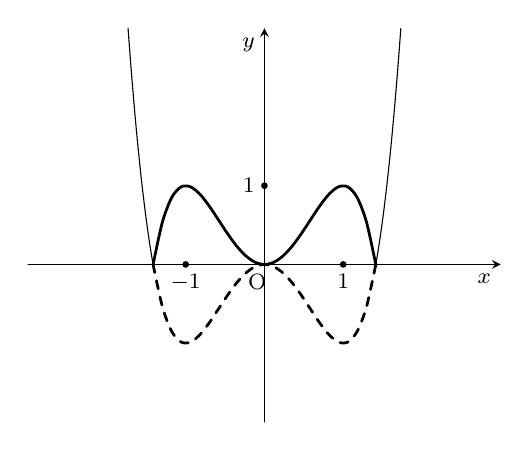
\begin{tikzpicture}[scale=1, font=\footnotesize, line join=round, line cap=round, >=stealth]
			\draw[-stealth] (-3,0)--(3,0) node[below left]{$x$};
			\draw[-stealth] (0,-2)--(0,3) node[below left]{$y$};
			\draw[dashed,line width=1.0pt,smooth,domain=-sqrt(2):sqrt(2)] plot(\x,{(\x)^4-2*(\x)^2});
			\draw[line width=1.0pt,smooth,domain=-sqrt(2):sqrt(2)] plot(\x,{-(\x)^4+2*(\x)^2});
			\draw[smooth,domain=sqrt(2):sqrt(3)] plot(\x,{(\x)^4-2*(\x)^2});
			\draw[smooth,domain=-sqrt(3):-sqrt(2)] plot(\x,{(\x)^4-2*(\x)^2});
			\draw[fill=black]
			(0.15,0)node[below left]{O}
			(-1,0) circle (1pt) node[below]{$-1$}
			(1,0) circle (1pt) node[below]{$1$}
			(0,1) circle (1pt) node[left]{$1$}
			;
		\end{tikzpicture}
		}
}
\end{ex}
\begin{ex}%Câu 8.%[Paul Hieu Nguyen]%[2D1K1-4]
	Cho phương trình $4(\sin^4x+\cos^4x)-8\left(\sin^6x+\cos^6x\right)-4\sin^24x=m$ trong đó $m$ là tham số. Để phương trình là vô nghiệm thì các giá trị thích hợp của $m$ là 
	\choice
	{$-1\leq m\leq 0$}
	{$-\dfrac{3}{2}\leq m\leq-1$}
	{$-2\leq m\leq-\dfrac{3}{2}$}
	{\True $m <-\dfrac{25}{4}$ hay $m>0$}
	\loigiai{
		$\sin^4x+\cos^4x=1-\dfrac{1}{2}\sin^22x$.\\
		$\sin^6x+\cos^6x=1-\dfrac{3}{4}\sin^22x$.\\
		Ta có phương trình: $3+\cos 4x-(5+3\cos 4x)-4(1-\cos^24x)=m$.\\
		Đặt $t=\cos 4x$, $t\in[-1;1]$, ta được phương trình $4t^2-2t-6=m$.\\
		Xét hàm số $f(t)=4t^2-2t-6$, $t\in[-1;1]$.\\
		$f'(t)=8t-2$.\\
		$f'(t)=8t-2=0\Leftrightarrow t=\dfrac{1}{4}$.\\
		Bảng biến thiên
		\begin{center}
			
\begin{tikzpicture}
			\tkzTabInit[nocadre=false,lgt=1.2,espcl=2.5,deltacl=0.6]
			{$t$ /1, $f'(t)$ /0.6, $f(t)$ /2}
			{$-1$,$\dfrac{1}{4}$,$1$}
			\tkzTabLine{,-,0,+,}
			\tkzTabVar{+/$0$,-/$-\dfrac{25}{4}$,+/$-4$}
			\end{tikzpicture}
		\end{center}
		Vậy $m <-\dfrac{25}{4}$ hay $m>0$.}
\end{ex}
\begin{ex}%Câu 9.%[Paul Hieu Nguyen]%[2D1G1-4]
	Phương trình $\left|x^2-2x\right|(|x|-1)=m$ (với $m$ là tham số thực) có tối đa bao nhiêu nghiệm thực?
	\choice
	{$3$}
	{\True $4$}
	{$5$}
	{$6$}
	\loigiai{
		Đặt $y=\left|x^2-2x\right|(|x|-1)=
		\heva{&(x^2-2x)(x-1),\,x\geq 2\\
			&(2x-x^2)(x-1),0\leq x<2\\
			&(x^2-2x)(-x-1),\,x<0.}$\\
		Khi đó, ta có 
		$y'=\heva{&3x^2-6x+2,\,x>2\\
			&-3x^2+6x-2,\,0<x<2\\
			&-3x^2+2x+2,\,x<0.}$ \\
		Ta được bảng biến thiên
		\begin{center}
			\begin{tikzpicture}[scale=0.9,yscale=.6,xscale=1.2]
			\begin{scope}[shift={(-.5,.5)}]
			\draw
			(0,0.5) rectangle +(14,-10)
			(0,-1.5)--+(0:14) (0,-3)--+(0:14) (1,0.5)--+(-90:10);
			\end{scope}
			\path
			(0,0) node{$x$} % <<< dòng 1
			++(0:1) node{$-\infty$}
			++(0:2) node{$\dfrac{1-\sqrt{7}}{3}$}
			++(0:2) node{$0$}
			++(0:2) node{$\dfrac{3-\sqrt{3}}{2}$}
			++(0:2) node{$2$}
			++(0:2) node{$\dfrac{3+\sqrt{3}}{2}$}
			++(0:2) node{$+\infty$}
			(0,-1.75) node{$y'$} % <<< dòng 2
			++(0:2) node{$-$}
			++(0:1) node{$0$}
			++(0:1) node{$+$}
			++(0:1) node{$||$}
			++(0:1) node{$-$}
			++(0:1) node{$0$}
			++(0:1) node{$+$}
			++(0:1) node{$||$}
			++(0:1) node{$-$}
			++(0:1) node{$0$}
			++(0:1) node{$+$}
			(0,-5.75) node{$y$} % <<< dòng 3
			++(0:1) +(90:2.5) node (I) {$+\infty$}
			++(0:2) +(-90:2.5) node (A) {$ $}
			++(0:2) +(-90:.5) node (B) {$0$}
			++(0:2) +(-90:1.5) node (C) {$ $}
			++(0:2) +(90:1.5) node (D) {$ $}
			++(0:2) +(-90:.5) node (E) {$0$}
			++(0:2) +(90:2.5) node (F) {$+\infty$}
			;
			\foreach \p/\q in {I/A,A/B,B/C,C/D,D/E,E/F}
			\draw[-stealth,blue] (\p)--(\q);
			\end{tikzpicture}
		\end{center}
		Vậy có nhiều nhất bốn nghiệm.}
\end{ex}
\begin{ex}%Câu 10.%[Paul Hieu Nguyen]%[2D1B1-4]
	Cho hàm số $y=f(x)$ xác định trên $\mathbb{R}\setminus\{0\}$, liên tục trên mỗi khoảng xác định và có bảng biến thiên sau
	\begin{center}
		
\begin{tikzpicture}
		\tkzTabInit[nocadre=false,lgt=1.2,espcl=2.5,deltacl=0.6]
		{$x$ /0.6, $y'$ /0.6, $y$ /2}
		{$-\infty$,$0$,$2$,$+\infty$}
		\tkzTabLine{,-,d,+,0,-,}
		\tkzTabVar{+/$+\infty$,-D-/$-2$/$-\infty$,+/$4$,-/$-\infty$}
		\end{tikzpicture}
	\end{center}
	Tìm tập hợp tất cả các giá trị thực của tham số $m$ sao cho phương trình $f(x)=m$ có ba nghiệm thực phân biệt. 
	\choice
	{$[-2;4]$}
	{$(-2;4)$}
	{\True $(-2;4]$}
	{$(-\infty;4]$}
	\loigiai{
		Dựa vào bảng biến thiên, ta có phương trình $f(x)=m$ có ba nghiệm thực phân biệt khi $m\in(-2;4]$.}
\end{ex}
\begin{ex}%Câu 11.%[Paul Hieu Nguyen]%[2D1G1-4]
	Cho hàm số $f(x)=\left(1-m^3\right)x^3+3x^2+(4-m)x+2$ với $m$ là tham số. Có bao nhiêu số nguyên $m\in[-2018;2018]$ sao cho $f(x)\geq 0$ với mọi giá trị $x\in[2;4]$. 
	\choice
	{$4037$}
	{$2021$}
	{$2019$}
	{\True $2020$}
	\loigiai{
		Ta có:
		\begin{eqnarray*}
			f(x)\geq0 &\Leftrightarrow&
			\left(1-m^3\right)x^3+3x^2+(4-m)x+2\ge0\\
			&\Leftrightarrow&
			(x+1)^3+(x+1)\ge(mx)^3+mx
		\end{eqnarray*}
		Xét hàm số $g(t)=t^3+t$ trên $\mathbb{R}$, có $g'(t)=3t^2+1>0$, $\forall t\in\mathbb{R}$.\\
		Do đó hàm số $g(t)$ đồng biến trên $\mathbb{R}$ \\
		$ \Rightarrow(1)\Leftrightarrow g(x+1)\geq g(mx)\Leftrightarrow x+1\geq mx $.\\
		Suy ra: $f(x)\geq 0$, $\forall x\in[2;4]\Leftrightarrow x+1\geq mx$, $\forall x\in[2;4]\Leftrightarrow m\leq\dfrac{x+1}{x}$, $\forall x\in[2;4]$.\\
		Nhận thấy: hàm số $h(x)=\dfrac{x+1}{x}$ nghịch biến trên đoạn $[2;4]$ \\
		$ \Rightarrow\min\limits_{[2;4]} h(x)=h(4)=\dfrac{5}{4} $ \\
		$ \Rightarrow m\leq h(x) $, $\forall x\in[2;4]\Leftrightarrow m\leq\min\limits_{[2;4]} h(x)\Leftrightarrow m\leq\dfrac{5}{4}$.\\
		Lại do $m$ nguyên thuộc đoạn $[-2018;2018]$ nên có $2020$ giá trị của $m$ thỏa mãn.}
\end{ex}
\begin{ex}%Câu 12.%[Paul Hieu Nguyen]%[2D1G1-4]
	Có bao nhiêu giá trị nguyên $m$ để phương trình $\left(8\sin^3x-m\right)^3=162\sin x+27m$ có nghiệm thỏa mãn $0<x<\dfrac{\pi}{3}$?
	\choice
	{\True $2$}
	{$3$}
	{Vô số}
	{$1$}
	\loigiai{
		Đặt $t=2\sin x$, với $0<x<\dfrac{\pi}{3}$ thì $t\in(0;\sqrt{3})$.\\
		Phương trình đã cho trở thành $\left(t^3-m\right)^3=81t+27m$.\\
		Đặt $u=t^3-m\Rightarrow t^3=u+m$.\\
		Khi đó ta được $\heva{&u^3=27(3t+m)\\&(3t)^3=27(u+m)}\Rightarrow u^3-(3t)^3=27(3t-u)\Leftrightarrow u^3+27u=(3t)^3+27\cdot 3t \quad (*)$.\\
		Xét hàm số $f(v)=v^3+27v$ liên tục trên $\mathbb{R}$ có nên hàm số đồng biến.\\
		Do đó $(*)\Leftrightarrow u=3t\Rightarrow t^3-3t=m \quad (1)$.\\
		Xét hàm số $f(t)=t^3-3t$ trên khoảng $(0;\sqrt{3})$.\\
		có $f'(t)=3t^2-3$; $f'(t)=0\Leftrightarrow t=1$.\\
		Bảng biến thiên
		\begin{center}
			
\begin{tikzpicture}
			\tkzTabInit[nocadre=false,lgt=1.2,espcl=2.5,deltacl=0.6]
			{$t$ /1, $f'(t)$ /0.6, $f(t)$ /2}
			{$0$,$1$,$\sqrt{3}$}
			\tkzTabLine{,-,0,+,}
			\tkzTabVar{+/$0$,-/$-2$,+/$0$}
			\end{tikzpicture}
		\end{center}
		Dựa vào bảng biến thiên ta thấy phương trình $(1)$ có nghiệm khi $-2\leq m<0$.\\
		Vậy có hai giá trị nguyên của $m$ thỏa yêu cầu bài toán.}
\end{ex}
\begin{ex}%Câu 13.%[Paul Hieu Nguyen]%[2D1B1-4]
	Với giá trị nào của $m$ để phương rình $x(x-3)^2=m-1$ có ba nghiệm phân biệt. 
	\choice
	{$m>1$}
	{$1\leq m\leq 5$}
	{$1<m<3$}
	{\True $1<m<5$}
	\loigiai{
		Xét hàm số $f(x)=x(x-3)^2=x^3-6x^2+9x$ trên $\mathbb{R}$ ta có:\\
		$f'(x)=3x^2-12x+9$.\\
		$f'(x)=0\Leftrightarrow 3x^2-12x+9=0\Leftrightarrow\hoac{&x=1\\&x=3.}$ \\
		Bảng biến thiên: 
		\begin{center}
			
\begin{tikzpicture}
			\tkzTabInit[nocadre=false,lgt=1.2,espcl=2.5,deltacl=0.6]
			{$x$ /0.6, $y'$ /0.6, $y$ /2}
			{$-\infty$,$1$,$3$,$+\infty$}
			\tkzTabLine{,+,0,-,0,+,}
			\tkzTabVar{-/$-\infty$,+/$4$,-/$0$,+/$+\infty$}
			\end{tikzpicture}
		\end{center}
		Dựa vào bảng biến thiên suy ra phương trình $x(x-3)^2=m-1$ có ba nghiệm phân biệt khi\\
		$0<m-1<4\Leftrightarrow 1<m<5$.}
\end{ex}
\begin{ex}%Câu 14.%[Paul Hieu Nguyen]%[2D1B1-4]
	Cho hàm số $y=f(x)$ có bảng biến thiên sau. Tìm $m$ để phương trình $f(x)=m$ có số nghiệm nhiều nhất. \begin{center}
		
\begin{tikzpicture}
		\tkzTabInit[nocadre=false,lgt=1.2,espcl=2.5,deltacl=0.6]
		{$x$ /0.6, $y'$ /0.6, $y$ /2}
		{$-\infty$,$-2$,$0$,$3$,$+\infty$}
		\tkzTabLine{,+,0,-,0,+,0,-,}
		\tkzTabVar{-/$-\infty$,+/$2$,-/$-5$,+/$0$,-/$-\infty$}
		\end{tikzpicture}
	\end{center}
	\choice
	{$m\in (-\infty;-5)$}
	{$m\in (-5;2)$}
	{$m\in (-\infty;0)$}
	{\True $m\in (-5;0)$ }
	\loigiai{
		Từ bảng biến thiên ta thấy phương trình $f(x)=m$ có số nghiệm nhiều nhất là $4$ khi và chỉ khi $m\in (-5;0)$.}
\end{ex}
\begin{ex}%Câu 15.%[Paul Hieu Nguyen]%[2D1B1-4]
	Cho hàm số $y=f(x)$ xác định, liên tục trên $\mathbb{R}$ và có bảng biến thiên sau 
	\begin{center}
		
\begin{tikzpicture}
		\tkzTabInit[nocadre=false,lgt=1.2,espcl=2.5,deltacl=0.6]
		{$x$ /0.6, $y'$ /0.6, $y$ /2}
		{$-\infty$,$-1$,$0$,$1$,$+\infty$}
		\tkzTabLine{,-,0,+,0,-,0,+,}
		\tkzTabVar{+/$+\infty$,-/$-1$,+/$0$,-/$-1$,+/$+\infty$}
		\end{tikzpicture}
	\end{center}
	Tìm tất cả các giá trị thực của tham số $m$ để phương trình $f(x)-1=m$ có đúng.\\
	hai nghiệm. 
	\choice
	{$m=-2, m\geq-1$}
	{$m>0, m=-1$}
	{\True $m=-2, m >-1$}
	{$-2<m <-1$}
	\loigiai{
		Ta có $f(x)-1=m\Leftrightarrow f(x)=m+1$. Từ bảng biến thiên suy ra phương trình có đúng hai nghiệm khi và chỉ khi $\hoac{&m+1=-1\\&m+1>0}\Leftrightarrow\hoac{&m=-2\\&m >-1}$.}
\end{ex}
\begin{ex}%Câu 16.%[Paul Hieu Nguyen]%[2D1B1-4]
	Tìm các giá trị của tham số $m$ để phương trình $x^3-3x=m^2+m$ có ba nghiệm phân biệt. 
	\choice
	{\True $-2<m<1$}
	{$-1<m<2$}
	{$m<1$}
	{$m >-21$}
	\loigiai{
		Xét hàm số $y=x^3-3x$.\\
		$y'=3x^2-3$.\\
		$y'=0\Leftrightarrow\hoac{&x=-1\Rightarrow y=2\\&x=1\Rightarrow y=-2.}$ \\
		Bảng biến thiên của hàm số $y=x^3-3x$ 
		\begin{center}
			
\begin{tikzpicture}
			\tkzTabInit[nocadre=false,lgt=1.2,espcl=2.5,deltacl=0.6]
			{$x$ /0.6, $y'$ /0.6, $y$ /2}
			{$-\infty$,$-1$,$1$,$+\infty$}
			\tkzTabLine{,+,0,-,0,+,}
			\tkzTabVar{-/$-\infty$,+/$2$,-/$-2$,+/$+\infty$}
			\end{tikzpicture}
		\end{center}
		Từ bảng biến thiên ta thấy phương trình $x^3-3x=m^2+m$ có ba nghiệm phân biệt khi\\
		$-2<m^2+m<2\Leftrightarrow\heva{&m^2+m-2<0\\&m^2+m+2>0 (\forall m\in\mathbb{R})}\Leftrightarrow-2<m<1$.}
\end{ex}
\begin{ex}%Câu 17.%[Paul Hieu Nguyen]%[2D1K1-4]
	Có bao nhiêu giá trị nguyên của tham số $m$ để phương trình $\dfrac{3}{4}\cos^22x+3\sin x\cdot\cos x-\dfrac{m}{4}+\dfrac{9}{4}=0$ có nghiệm?
	\choice
	{$5$}
	{$11$}
	{$9$}
	{\True $13$}
	\loigiai{
		Ta có 
		\begin{eqnarray*}
		\dfrac{3}{4}\cos^2 2x+3\sin x\cdot\cos x-\dfrac{m}{4}+\dfrac{9}{4}=0
		&\Leftrightarrow&
		-\dfrac{3}{4}\sin^2 2x+\dfrac{3}{2}\sin 2x+3-\dfrac{m}{4}=0\\
		&\Leftrightarrow&
		-3\sin^2 2x+6\sin2x+12=m \quad (*)
		\end{eqnarray*}
		Đặt $t=\sin 2x, t\in[-1;1]$ khi đó ta có phương trình $-3t^2+6t+12=m$.\\
		Bài toán trở thành tìm $m$ để phương trình có nghiệm $t\in[-1;1]$.\\
		Xét hàm số $f(t)=-3t^2+6t+12; f'(t)=-6t+6$.\\
		$f'(t)=0\Leftrightarrow t=1$.\\
		Bảng biến thiên
		\begin{center}
			
\begin{tikzpicture}
			\tkzTabInit[nocadre=false,lgt=1.2,espcl=2.5,deltacl=0.6]
			{$t$ /0.6, $f'(t)$ /0.6, $f(t)$ /1.5}
			{$-1$,$1$}
			\tkzTabLine{,+,}
			\tkzTabVar{-/$-3$,+/$15$}
			\end{tikzpicture}
		\end{center}
		Phương trình có nghiệm khi $3\leq m\leq 15$.\\
		Vậy có $13$ giá trị nguyên của $m$ để phương trình có nghiệm.}
\end{ex}
\begin{ex}%Câu 18.%[Paul Hieu Nguyen]%[2D1G1-4]
	(THPT SỐ 02 AN NHƠN BÌNH ĐỊNH LẦN 02 NĂM 2018) Cho phương trình $\sin 2x-\cos 4x+8\sqrt{2}\left|\sin\left(x+\dfrac{\pi}{4}\right)\right|=m+8\sqrt{2\cos^22x+m}$. Có bao nhiêu giá trị nguyên của tham số $m$ để phương trình trên có đúng một nghiệm thuộc khoảng $\left[0;\dfrac{7\pi}{12}\right)$?
	\choice
	{\True $1$}
	{$3$}
	{$2$}
	{$4$}
	\loigiai{
		\begin{eqnarray*}
		& & \sin 2x-\cos 4x+8\sqrt{2}\left|\sin\left(x+\dfrac{\pi}{4}\right)\right|=m+8\sqrt{2\cos^22x+m} \\
		&\Leftrightarrow&
		\sin 2x+1-2\cos^22x+8\left|\sin x+\cos x\right|=m+8\sqrt{2\cos^22x+m} \\
		&\Leftrightarrow&
		\left(\sin x+\cos x\right)^2+8\left|\sin x+\cos x\right|=\left(2\cos^22x+m\right)+8\sqrt{2\cos^22x+m} \quad (1)
		\end{eqnarray*}
		Xét hàm số: $f(t)=t^2+8t$, $f'(t)=2t+8>0$, $\forall t\geq 0$ \\
		$ \Rightarrow $ Hàm số $f(t)$ đồng biến trên $[0;+\infty)$.
		\begin{eqnarray*}
		(1)
		&\Leftrightarrow&
		f\left(\left|\sin x+\cos x\right|\right)=f\left(\sqrt{2\cos^22x+m}\right) \\
		&\Leftrightarrow&
		\left|\sin x+\cos x\right|=\sqrt{2\cos^22x+m} \\
		&\Leftrightarrow&
		\sin 2x+1=2\cos^22x+m \\
		&\Leftrightarrow&
		m=2\sin^22x+\sin 2x-1
		\end{eqnarray*}
		Ta có: $x\in\left[0;\dfrac{7\pi}{12}\right)\Leftrightarrow 2x\in\left[0;\dfrac{7\pi}{6}\right)\Rightarrow\sin 2x\in\left(-\dfrac{1}{2};1\right]$.\\
		Xét $g(u)=2u^2+u-1$ với $u\in\left(-\dfrac{1}{2};1\right]$.\\
		Nhận xét:\\
		$g'(u)=4u+1$, $g'(u)=0\Leftrightarrow u=-\dfrac{1}{4}$ 
		\begin{center}
			
\begin{tikzpicture}
			\tkzTabInit[nocadre=false,lgt=1.2,espcl=2.5,deltacl=0.6]
			{$t$ /1, $g'(u)$ /0.6, $g(u)$ /2}
			{$-\dfrac{1}{2}$,$-\dfrac{1}{4}$,$1$}
			\tkzTabLine{,-,0,+,}
			\tkzTabVar{+/$-1$,-/$-\dfrac{9}{8}$,+/$2$}
			\end{tikzpicture}
		\end{center}
		Phương trình $m=g(u)$ ứng với $1$ nghiệm $u\in\left(\dfrac{-1}{2};0\right)\cup\{1\}$ cho $1$ nghiệm $x\in\left[0;\dfrac{7\pi}{12}\right)$.\\
		Phương trình $m=g(u)$ ứng với $1$ nghiệm $u\in[0;1)$ cho $2$ nghiệm $x\in\left[0;\dfrac{7\pi}{12}\right)$.\\
		Ta có: $g(0)=-1$.\\
		Dựa vào BBT, phương trình có đúng $1$ nghiệm $x\in\left[0;\dfrac{7\pi}{12}\right)\Leftrightarrow m=2$.\\
		Có $1$ giá trị nguyên của $m$ thỏa yêu cầu.}
\end{ex}
\begin{ex}%Câu 19.%[Paul Hieu Nguyen]%[2D1B1-4]
	Với giá trị nào của $k$ thì phương trình $-x^3+3x+2-k=0$ có $3$ nghiệm phân biệt. 
	\choice
	{$-1<k<1$}
	{$\hoac{&k<0\\&k>4}$}
	{$0\leq k\leq 4$}
	{\True $0<k<4$}
	\loigiai{
		Ta có: $-x^3+3x+2-k=0\Leftrightarrow k=-x^3+3x+2$.\\
		Đặt $f(x)=-x^3+3x+2\Rightarrow f'(x)=-3x^2+3=0\Leftrightarrow x=\pm 1$.\\
		Bảng biến thiên
		\begin{center}
			
\begin{tikzpicture}
			\tkzTabInit[nocadre=false,lgt=1.2,espcl=2.5,deltacl=0.6]
			{$x$ /0.6, $y'$ /0.6, $y$ /2}
			{$-\infty$,$-1$,$1$,$+\infty$}
			\tkzTabLine{,-,0,+,0,-,}
			\tkzTabVar{+/$+\infty$,-/$0$,+/$4$,-/$-\infty$}
			\end{tikzpicture}
		\end{center}
		Dựa vào bảng biến thiên để đường thẳng $y=k$ cắt đồ thị hàm số $f(x)$ tại $3$ điểm phân biệt khi $0<k<4$.}
\end{ex}
\begin{ex}%Câu 20.%[Paul Hieu Nguyen]%[2D1K1-4]
	Tìm $m$ để phương trình $x^6-3x^2-2=m$ có hai nghiệm phân biệt. 
	\choice
	{$\hoac{&m=4\\&m\geq 2}$}
	{$m >-2$}
	{$-4<m <-2$}
	{\True $\hoac{&m=-4\\&m >-2}$}
	\loigiai{
		Ta có số nghiệm của phương trình $x^6-3x^2-2=m$ là số giao điểm của đồ thị hàm số $y=x^6-3x^2-2$ và đường thẳng $y=m$.\\
		Xét hàm số $y=x^6-3x^2-2$ có:\\
		+ Tập xác định: $\mathscr{D}=\mathbb{R}$.\\
		+ $y'=6x^5-6x; y'=0\Leftrightarrow 6x\left(x^4-1\right)=0\Leftrightarrow 6x\left(x^2-1\right)\left(x^2+1\right)=0\Leftrightarrow\hoac{&x=0\\&x=\pm 1.}$ \\
		+ Bảng biến thiên 
		\begin{center}
			
\begin{tikzpicture}
			\tkzTabInit[nocadre=false,lgt=1.2,espcl=2.5,deltacl=0.6]
			{$x$ /0.6, $y'$ /0.6, $y$ /2}
			{$-\infty$,$-1$,$0$,$1$,$+\infty$}
			\tkzTabLine{,-,0,+,0,-,0,+,}
			\tkzTabVar{+/$+\infty$,-/$-4$,+/$-2$,-/$-4$,+/$+\infty$}
			\end{tikzpicture}
		\end{center}
		Dựa vào bảng biến thiên, ta thấy phương trình $x^6-3x^2-2=m$ có hai nghiệm phân biệt\\
		$ \Leftrightarrow\hoac{&m=-4\\&m >-2.} $ }
\end{ex}
\Closesolutionfile{ans}